% Copyright 2004 by Till Tantau <tantau@users.sourceforge.net>.
%
% In principle, this file can be redistributed and/or modified under
% the terms of the GNU Public License, version 2.
%
% However, this file is supposed to be a template to be modified
% for your own needs. For this reason, if you use this file as a
% template and not specifically distribute it as part of a another
% package/program, I grant the extra permission to freely copy and
% modify this file as you see fit and even to delete this copyright
% notice. 

\documentclass{beamer}
\usepackage{url}
\usepackage{algorithm} 
\usepackage{algorithmic}
\usepackage{float}
%%

  
%\floatname{algorithm}{算法}  
%\renewcommand{\algorithmicrequire}{\textbf{输入:}}  
%\renewcommand{\algorithmicensure}{\textbf{输出:}}  
%
%\renewcommand{\algorithmicrequire}{\textbf{Input:}}  % Use Input in the format of Algorithm  
%\renewcommand{\algorithmicensure}{\textbf{Output:}} % Use Output in the format of Algorithm  


% There are many different themes available for Beamer. A comprehensive
% list with examples is given here:
% http://deic.uab.es/~iblanes/beamer_gallery/index_by_theme.html
% You can uncomment the themes below if you would like to use a different
% one:
%\usetheme{AnnArbor}
%\usetheme{Antibes}
%\usetheme{Bergen}
%\usetheme{Berkeley}
%\usetheme{Berlin}
%\usetheme{Boadilla}
%\usetheme{boxes}
%\usetheme{CambridgeUS}
%\usetheme{Copenhagen}
%\usetheme{Darmstadt}
%\usetheme{default}
%\usetheme{Frankfurt}
%\usetheme{Goettingen}
%\usetheme{Hannover}
%\usetheme{Ilmenau}
%\usetheme{JuanLesPins}
%\usetheme{Luebeck}
\usetheme{Madrid}
%\usetheme{Malmoe}
%\usetheme{Marburg}
%\usetheme{Montpellier}
%\usetheme{PaloAlto}
%\usetheme{Pittsburgh}
%\usetheme{Rochester}
%\usetheme{Singapore}
%\usetheme{Szeged}
%\usetheme{Warsaw}
%\usepackage{movie15}

\title{Research Summary}

% A subtitle is optional and this may be deleted
% subtitle{Optional Subtitle}

\author{Jiawei Sun}
% - Give the names in the same order as the appear in the paper.
% - Use the \inst{?} command only if the authors have different
%   affiliation.

\institute[sunmessi@umich.edu] % (optional, but mostly needed)
{\\


  \textbf{Electrical and Computer Engineering}\\
  \\
  \textbf{University of Michigan}\\

%   \and
% \inst{2}%
%  Department of Theoretical Philosophy\\
%   University of Elsewhere
 }
%% - Use the \inst command only if there are several affiliations.
%% - Keep it simple, no one is interested in your street address.

\date{October, 2019}
% - Either use conference name or its abbreviation.
% - Not really informative to the audience, more for people (including
%   yourself) who are reading the slides online

%\subject{Theoretical Computer Science}
% This is only inserted into the PDF information catalog. Can be left
% out. 

% If you have a file called "university-logo-filename.xxx", where xxx
% is a graphic format that can be processed by latex or pdflatex,
% resp., then you can add a logo as follows:

% \pgfdeclareimage[height=0.5cm]{university-logo}{university-logo-filename}
% \logo{\pgfuseimage{university-logo}}

% Delete this, if you do not want the table of contents to pop up at
% the beginning of each subsection:
\AtBeginSubsection[]
{
  \begin{frame}<beamer>{Outline}
    \tableofcontents[currentsection,currentsubsection]
  \end{frame}
}

% Let's get started
\begin{document}

\begin{frame}
  \titlepage
\end{frame}

\begin{frame}{Outline}
  \tableofcontents
  % You might wish to add the option [pausesections]
\end{frame}

% Section and subsections will appear in the presentation overview
% and table of contents.
%\section{PCA Principle Component Analysis}
%
%\subsection{View of PCA}
%
%
%\begin{frame}{View of PCA}{Minimizing the MSE}
%  \begin{itemize}
%  \item {
%  	$ x \in {R^n} $, and $ E\{ x\}  = 0 $ 
%  }
%  \item{
%  	Project x in n dimension to m dimension subspace,$m < n$.
%  }
%  \item {
%    Choose a set of bases which are orthonormal, $ W = [{w_1},{w_2},...,{w_m}] $.
%  }
%  \item{
%  	Project x to $ {w_i} $, the scalar in $ {w_i} $ is $ w_i^Tx $, the coordinate in $ {w_i} $ is $ (w_i^Tx){w_i} $.
%  }
%  \item{
%  	The coordinate in the m dimension subspace 
%  	\[Px = \sum\limits_{i = 1}^m {(w_i^Tx){w_i}}  = \sum\limits_{i = 1}^m {{w_i}w_i^Tx = W{W^T}x} \]
%  }
%  \end{itemize}
%\end{frame}
%
%
%\begin{frame}{View of PCA}{Minimizing the MSE}
%  \begin{itemize}
%  \item {
%  	Projecting x to m dim loses $n-m$ dimension information.
%  }
%  \item{
%  	If we want to preserve more information, we should minimize the Mean-Square error.
%  	\[e_{MSE}^{\min } = E\left\{ {{{\left\| {x - Px} \right\|}^2}} \right\}\]
%  }
%  \item{
%  	PCA can be posed as: finding a subspace that minimizes the MSE
%  	\[\mathop {\arg \min }\limits_W {J_{MSE}}(W) = E\left\{ {{{\left\| {x - Px} \right\|}^2}} \right\},s.t.,{\rm{ }}{W^T}W = I\]
%  }
%  \end{itemize}
%\end{frame}
%
%
%\begin{frame}{View of PCA}{Minimizing the MSE}
%  \begin{itemize}
%  \item {
%	\[{J_{MSE}}(W) = E\left\{ {{x^T}x} \right\} - E\left\{ {{x^T}Px} \right\}\]
%	\[\min {J_{MSE}}(W) \to \max E\left\{ {{x^T}Px} \right\}\]
%  }
%  \item{
%  	We can simplify PCA to
%  	\[\mathop {\arg \max }\limits_W E\{ {x^T}W{W^T}x\} ,s.t.,{W^T}W = I\]
%  }
%  \item{
%  	Lagrange multipliers method
%  	\[L(W,\lambda ) = E\{ {x^T}W{W^T}x\}  + \lambda (I - {W^T}W)\]
%  }
%  \item{
%  	Solve the derivative of $ {w_i} $
%  	\[\frac{{\partial L(W,\lambda )}}{{\partial {w_i}}} = 2E\{ x{x^T}\} {w_i} - 2{\lambda _i}{w_i}{\rm{, }}i = 1,2,...,m\]
%  }
%  \end{itemize}
%\end{frame}
%
%
%\begin{frame}{View of PCA}{Minimizing the MSE}
%  \begin{itemize}
%	\item{
%  		Let the derivative equal 0
%  		\[E\{ x{x^T}\} {w_i} = {\lambda _i}{w_i}{\rm{, }}i = 1,2,...,m\]
%  		$ {w_i} $ is the eigenvector of $ E\{ x{x^T}\} $, $ \lambda _i $ is the eigenvalue.
%    }
%  
%	\item{
%   When n is very large, it is demanding to eigenvalue decomposition.
%  }
%   \item{
%   How to deal with it?
%  }
%  \end{itemize}
%\end{frame}
%
%
%\subsection{Solve EVD}
%\begin{frame}{Solve EVD}{Power Method}
% \begin{itemize}
%  	\item{
%  		Assume $ {\lambda _1} > {\lambda _2} > ...>{\lambda _n} $ are the m eigenvalues of $ E\{ x{x^T}\} = A $ and $ {v _1} > {v _2} > ...>{v _n} $ are the corresponding eigenvectors. \cite{4}
%  	} 
%  	\item{
%  		Choose a random nonzero vector $ {x_0} $ in $ {R^n} $,
%   	}
%   	\item{
%   	
%  		\[\begin{array}{c}
%{x_1} = A{x_0} = {A^1}{x_0}\\
%{x_2} = A{x_1} = {A^2}{x_0}\\
% \vdots \\
%{x_k} = A{x_{k - 1}} = {A^k}{x_0}
%\end{array}\]
%  }
%  \item{
%  When k is large enough, $ {x_k} $ is the eigenvector of A.
%  }
% \end{itemize}
%\end{frame}
%
%\begin{frame}{Solve EVD}{Power Method}
%	\begin{itemize}
%		\item{
%  			Let us prove it.
%  		}
%  		\item{
%  	$ {x_0} $ is the linear combination of v
%  	\[{x_0} = {c_1}{v_1} + {c_2}{v_2} + ... + {c_n}{v_n}\]
%  }
%  \item{
%  \[\begin{array}{c}
%{A^k}{x_0} = {c_1}{A^k}{v_1} + {c_2}{A^k}{v_2} + ... + {c_n}{A^k}{v_n}\\
% = {c_1}\lambda _1^k{v_1} + {c_2}\lambda _2^k{v_2} + ... + {c_n}\lambda _n^k{v_n}\\
% = \lambda _1^k({c_1}{v_1} + {c_2}{(\frac{{{\lambda _2}}}{{{\lambda _1}}})^k}{v_2} + ... + {(\frac{{{\lambda _n}}}{{{\lambda _1}}})^k}{v_n})
%\end{array}\]
%}
%\item{
%	When k is larger enough,  $ {(\frac{{{\lambda _i}}}{{{\lambda _1}}})^k} \approx 0 $
%  \[{A^k}{x_0} \approx {c_1}\lambda _1^k{v_1}\]
%  }
%	\end{itemize}
%\end{frame}
%
%
%
%\begin{frame}{Solve EVD}{Oja Method}
%	\begin{itemize}
%	  \item{
%	 	We develop a cost function which is used to measure how well current parameter values work. We can find the minimum point of the cost function by iteratively taking steps in the opposite direction of current slope.
%	  }
%	  \item{
%	  	Define the process of gradient descent as
%	  	\[W(t + 1) = W(t) + \Delta W(t)\]
%	  	where
%	  	\[\Delta W(t) =  - \alpha \frac{{\partial {J_{MSE}}(W)}}{{\partial W(t)}}\]
%	  	$ \Delta W(t) $ is the step which we take walking along the gradient,$ \alpha $ is the size of steps. 
%	  }
%	\end{itemize}
%
%\end{frame}
%
%
%
%\begin{frame}{Solve EVD}{Oja Method}
%	\begin{itemize}
%		\item{
%			Looking at the view of MSE minimization, our cost function:
%			\[\begin{array}{c}
%{\left\| {x - W{W^T}x} \right\|^2} = {\left\| {x - \sum\limits_{i = 1}^m {w_i^T(t)x{w_i}(t)} } \right\|^2}\\
% = {\left\| {x - \sum\limits_{i = 1}^m {{y_i}{w_i}(t)} } \right\|^2}
%\end{array}\]
%			
%		}
%		\item{
%		Solve the derivative
%		\[\begin{array}{l}
%\Delta {w_i}(t) = \gamma {y_i}[x - \sum\limits_{i = 1}^m {{y_i}{w_i}(t)} ]\\
%\Delta W = \gamma (x{x^T} - W{W^T}x{x^T})W
%\end{array}\]
%		}
%	\end{itemize}
%
%\end{frame}

\section{Differential Microphones Arrays based on Differential Equation}

\subsection{Linear DMA}

\begin{frame}{Linear DMA}{Signal Model}
\begin{itemize}
\item The basic mode of an uniform linear array (ULA) with M omnidirectional microphones is
\begin{equation}
  \begin{align}
\label{eq:signal mode}
   {{y}_{m}}(k)&={{x}_{m}}(k)+{{v}_{m}}(k) \\ 
 & ={x}(k-t-{{\tau }_{m}})+{{v}_{m}}(k),m=1,2,...,M  
\end{align}
\end{equation}
\begin{figure}[ht]
		%\centering
		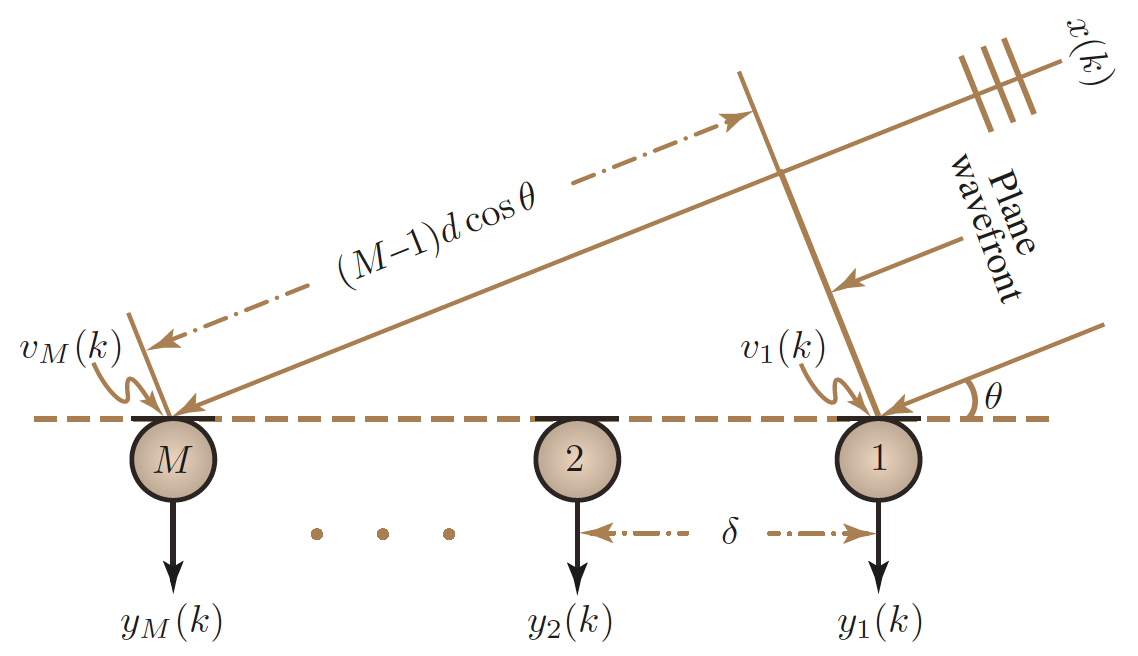
\includegraphics[scale=0.34]{DMA.3.png}
		\caption{Uniform Linear Array} 
		\label{LDMA}	
	\end{figure}
\end{itemize}	
\end{frame}

\begin{frame}{Linear DMA}{Signal Model}
\begin{itemize}
\item
where ${{x}_{m}}(k)$ is the source signal, $ t $ is the time which it takes form the signal to  the first microphone, ${{\tau }_{m}}$ is the  delay between the mth and the first microphones. \cite{6}
\item
In the STFT domain,\eqref{eq:signal mode} can be expressed as
\begin{equation}
 {{Y}_{m}}(\omega )=X(\omega ){{e}^{-j(m-1)\omega {{\tau }_{0}}\cos \theta }}+{{V}_{m}}(\omega )
\end{equation}

\end{itemize}	
\end{frame}


\begin{frame}{Linear DMA}{Signal Model}
\begin{itemize}
\item{
In vectors form, we get
\begin{align}
  y(\omega )&={{\left[ {{Y}_{1}}(\omega ),{{Y}_{2}}(\omega ),...,{{Y}_{M}}(\omega ) \right]}^{T}} \\ 
 & =d(\omega ,\cos \theta )\text{X}(\omega )+v(\omega )  
\end{align}
where
\begin{equation}
d(\omega ,\cos \theta )={{\left[ 1,{{e}^{-j\omega {{\tau }_{0}}\cos \theta }},...,{{e}^{-j(M-1)\omega {{\tau }_{0}}\cos \theta }} \right]}^{T}}
\end{equation}
is the phase-delay vector of length M.
}
\item{
In order to recover the desired signal $X(\omega )  $ from $ y(\omega ) $, a complex weight $ H_m^* (\omega )  $ is designed and applied to the output of each microphone. Mathematically, the beamformer’s output is

\begin{equation}
Z(\omega )=\sum\limits_{m=1}^{M}{H_{m}^{*}(\omega ){{Y}_{\text{m}}}(\omega )}={{h}^{T}}(\omega )y(\omega )
\end{equation}

}
\end{itemize}
	
\end{frame}

\begin{frame}{Linear DMA}{Beampatterns}
\begin{itemize}
\item{
Mathematically, beampattern of a Nth-order DMA is written as
\begin{align}
   B[h(\omega ),\theta ]&={{d}^{H}}(\omega ,\cos \theta )h(\omega ) \\ 
 & =\sum\limits_{m=1}^{M}{{{H}_{m}}(\omega ){{e}^{j(m-1)\omega {{\tau }_{0}}\cos \theta }}} 
\label{eq:Beampatterns} 
\end{align}
Simplify \eqref{eq:Beampatterns} by McLaughlin expanion, we get
\begin{equation}
\label{eq:Beampatterns2} 
{{B}_{N}}(\theta )=\sum\limits_{n=0}^{N}{{{a}_{N,n}}{{\cos }^{n}}\theta }
\end{equation}
where $ {{\rm{a}}_{N,n}} $,$ n=0,1,...,N$ are real coefficients.

}

\end{itemize}
	
\end{frame}

\begin{frame}{Linear DMA}{Beampatterns}
\begin{itemize}
\item{
In the direction of the desired signal, i.e., $\theta  = {0^ \circ }$, the directivity pattern must be equal to 1. Therefore, we should have
\begin{equation}
\sum\limits_{n=0}^{N}{{{a}_{N,n}}}=1
\end{equation}

}
\end{itemize}
	
\end{frame}


\begin{frame}{Linear DMA}{Linear equations solves beampattern coefficients}
\begin{itemize}
\item{
The second-order directivity patterns have the form:
\begin{equation}
{{B}_{2}}(\theta )=(1-{{a}_{2,1}}-{{a}_{2,2}})+{{a}_{2,1}}\cos \theta +{{a}_{2,2}}{{\cos }^{2}}\theta 
\end{equation}
and they have 2 nulls at the angle ${{\theta }_{1}}$ and ${{\theta }_{2}}$, so we can write differential equation about ${{\rm{a}}_{2,1}}$ and ${{\rm{a}}_{2,2}}$,
\begin{equation}
\left\{ \begin{array}{*{35}{l}}
   (1-{{a}_{2,1}}-{{a}_{2,2}})+{{a}_{2,1}}\cos {{\theta }_{1}}+{{a}_{2,2}}{{\cos }^{2}}{{\theta }_{1}}=0  \\
   (1-{{a}_{2,1}}-{{a}_{2,2}})+{{a}_{2,1}}\cos {{\theta }_{2}}+{{a}_{2,2}}{{\cos }^{2}}{{\theta }_{2}}=0  \\
\end{array} \right.
\end{equation}
}
\item{
By solving the equation, the most important shapes of patterns are as follows
\begin{itemize}
	\item Dipole: $a_{2,1}  = 0 $, $a_{2,2}  = 1 $, nulls at $ \cos \theta  = 0 $.
	\item Cardioid: $a_{2,1} = a_{2,2} = \frac{1}{2} $, nulls at $ \cos \theta  = 0 $ and $ \cos \theta  = -1 $.

\end{itemize}
}
\end{itemize}
	
\end{frame}

\begin{frame}{Linear DMA}{Linear equations solves beampattern coefficients}
\begin{itemize}
\item{
As for Nth-order directivity patterns, they have N nulls at $ {\theta _1} $, $ {\theta _2} $,...,$ {\theta _N} $ and the directivity pattern is equal to 1 in the direction of the desired signal. Based on the known conditions, we get
\begin{equation}
\left\{ \begin{matrix}
   \sum\limits_{n=0}^{N}{{{a}_{N,n}}=1}  \\
   \sum\limits_{n=0}^{N}{{{a}_{N,n}}{{\cos }^{n}}{{\theta }_{1}}=0}  \\
   \sum\limits_{n=0}^{N}{{{a}_{N,n}}{{\cos }^{n}}{{\theta }_{2}}=0}  \\
   \vdots   \\
   \sum\limits_{n=0}^{N}{{{a}_{N,n}}{{\cos }^{n}}{{\theta }_{N}}=0}  \\
\end{matrix} \right.
\end{equation}
Solve the simultaneous linear equations and get ${a_{N,0}}$, ${a_{N,2}}$,...,${a_{N,N}}$.
}
\end{itemize}
	
\end{frame}

\begin{frame}{Linear DMA}{Differential equations solves beampattern coefficients}
\begin{itemize}
\item{
By \eqref{eq:Beampatterns2} and the multiple-angle formula
\begin{equation}
{{\cos }^{n}}\theta =\frac{1}{{{2}^{n}}}\sum\limits_{k=0}^{n}{C_{n}^{k}\cos (2k-n)\theta }
\end{equation}

we get,
\begin{equation}
\label{eq:b0}
 {{B}_{N}}(\theta )=\sum\limits_{n=0}^{N}{{{b}_{N,n}}\cos n\theta }
\end{equation}
}
\end{itemize}
	
\end{frame}


\begin{frame}{Linear DMA}{Differential equations solves beampattern coefficients}
\begin{itemize}
\item{
Take the first-order equations as example, it is written as
\begin{equation}
\label{eq:b1}
  {{B}_{1}}(\theta )\text{=}{{b}_{1,0}}+{{b}_{1,1}}\cos \theta 
\end{equation}
As for a second-order constant coefficient differential equation,its corresponding characteristic equation is 
\begin{equation}
\label{eq:d1}
 {{y}^{(2)}}+{{n}^{2}}y=0
\end{equation}
\begin{equation}
 {{r}^{2}}+{{n}^{2}}=0
\end{equation}
so $r=\pm ni$, and its general solution is 
\begin{equation}
\label{eq:solution of d1}
y={{C}_{1}}\cos (n\theta )+{{C}_{2}}\sin (n\theta )
\end{equation}
}
\end{itemize}
	
\end{frame}

\begin{frame}{Linear DMA}{Differential equations solves beampattern coefficients}
\begin{itemize}
\item{
Characteristic equation of a Nth-order constant coefficient differential equation corresponding to Nth-order DMA is
\begin{equation}
  r({{r}^{2}}+{{1}^{2}})({{r}^{2}}+{{2}^{2}})\ldots ({{r}^{2}}+{{N}^{2}})=0
\end{equation}
To solve $(2N+1)$th-order differential equation needs 2N+1 initial conditions.
}
\end{itemize}
	
\end{frame}

\begin{frame}{Linear DMA}{Differential equations solves beampattern coefficients}
\begin{itemize}
\item{
The directivity pattern must be equal to 1.
\begin{equation}
 {{B}_{N}}({{0}^{{}^\circ }})=1
\end{equation}
Nth-order directivity patterns have N nulls at $ {\theta _1} $, $ {\theta _2} $,...,$ {\theta _N} $,
\begin{equation}
{{B}_{N}}({{\theta }_{1}})=0,{{B}_{N}}({{\theta }_{2}})=0,\ldots ,{{B}_{N}}({{\theta }_{N}})=0
\end{equation}
Its first derivative only exists $ \sin (n\theta ) $ and so on we can get the rest N initial condition,
\begin{equation}
B_{N}^{(1)}(0)=0,B_{N}^{(1)}(\pi )=0,B_{N}^{(2)}(\frac{\pi }{2})=0,B_{N}^{(2)}(\frac{3\pi }{2})=0...
\end{equation}
}
\end{itemize}
	
\end{frame}


\subsection{Circular DMA}

\begin{frame}{Circular DMA}{Beampattern}
\begin{itemize}
\item{
The beampattern of CDMA is defined as 
\begin{equation}
\label{eq:CDMA}
{{B}_{N}}(\theta )=\sum\limits_{n=0}^{N}{{{a}_{N,n}}{{\cos }^{n}}(\theta -{{\theta }_{s}})}
\end{equation}
where $ {{\rm{a}}_{N,n}} $,$ n=0,1,...,N$ are real coefficients. In the direction of the desired signal, i.e., $\theta ={{\theta }_{s}}$, the directivity pattern must be equal to 1 \cite{7}.
}

\begin{figure}[ht]
		%\centering
		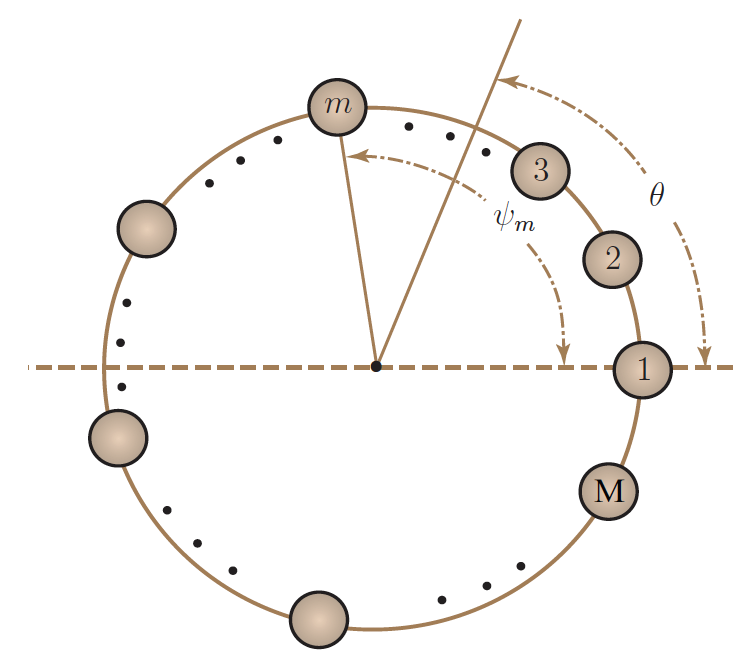
\includegraphics[scale=0.25]{3.png}
		\caption{Circular DMA} 
		\label{Circular DMA}	
	\end{figure}
\end{itemize}
	
\end{frame}

\begin{frame}{Circular DMA}{Differential Equations Solve Circular DMA}
\begin{itemize}
\item{
By \eqref{eq:CDMA} and the multiple-angle formula
\begin{align}
  {{B}_{N}}(\theta -{{\theta }_{s}}) &=\sum\limits_{n=0}^{N}{{{b}_{N,n}}\cos n(\theta -{{\theta }_{s}})} \\ 
 & =\sum\limits_{n=0}^{N}{{{b}_{N,n}}\cos n{{\theta }_{s}}\cos n\theta +{{b}_{N,n}}\sin n{{\theta }_{s}}\sin n\theta }  
\end{align}
Take the first-order equations as example, it is writtens as
\begin{equation}
\label{eq:CDMA1}
{{B}_{1}}(\theta -{{\theta }_{s}})={{b}_{1,0}}+{{b}_{1,1}}\cos {{\theta }_{s}}\cos \theta +{{b}_{1,1}}\sin {{\theta }_{s}}\sin \theta 
\end{equation}
When ${{b}_{1,0}}=C$, ${{C}_{1}}={{b}_{1,1}}\cos {{\theta }_{s}}$, ${{C}_{2}}={{b}_{1,1}}\sin {{\theta }_{s}}$, the solution of this differential equation is equal to \eqref{eq:CDMA1}.
}
\end{itemize}
	
\end{frame}

\begin{frame}{Circular DMA}{Differential Equations Solve Circular DMA}
\begin{itemize}
\item{
To solve $(2N+1)$th-order differential equation needs 2N+1 initial conditions. 
\begin{equation}
{{B}_{N}}({{\theta }_{s}})=1
\end{equation}
Nth-order directivity patterns have N nulls at ${{\theta }_{1}}-{{\theta }_{s}}$, ${{\theta }_{2}}-{{\theta }_{s}}$,...,${{\theta }_{N}}-{{\theta }_{s}}$,
\begin{equation}
{{B}_{N}}({{\theta }_{1}}-{{\theta }_{s}})=0,{{B}_{N}}({{\theta }_{2}}-{{\theta }_{s}})=0,\ldots ,{{B}_{N}}({{\theta }_{N}}-{{\theta }_{s}})=0
\end{equation}
Besides, we can get the rest N initial conditions,
\begin{equation}
\begin{align}
  & B_{N}^{(1)}({{\theta }_{s}})=0,B_{N}^{(1)}({{\theta }_{s}}+\pi )=0, \\ 
 & B_{N}^{(2)}({{\theta }_{s}}+\frac{\pi }{2})=0,B_{N}^{(2)}({{\theta }_{s}}+\frac{3\pi }{2})=0... \\ 
\end{align}
\end{equation}

}
\end{itemize}
	
\end{frame}



\section{Distributed Algorithms of PCA}

\subsection{Backgrounding}


\begin{frame}{Backgrounding}{Overview}
	 \begin{itemize}
	 	\item{
	 	Why we need Distributed Algorithms of PCA (D-PCA)?
	 	}
	 	\begin{enumerate}
  			\item data are collected/stored in a distributed network
  			\item memory limitation
  			\item privacy issue
  			\item parallel clusters
		\end{enumerate}
		
		\item{
		How D-PCA work for parallel processors?
		\begin{enumerate}
  			\item each node calculates its local value of PCA
  			\item communicate with its neighbor nodes
  			\item update with a weighted average of its neighbors’ values
		\end{enumerate}
		}
		\item{
		Application
		\begin{enumerate}
  			\item classify word documents
  			\item array processing
		\end{enumerate}

		}
	 \end{itemize}

\end{frame}

\begin{frame}{Backgrounding}{Two Types of Data Model}
	 \begin{itemize}
		\item{
			The designs of D-PCA algorithms differ in how data are divided in the network:
			\begin{enumerate}
			  \item Distributed columns observations (DCO)
			  \item Distributed rows observations (DRO)
			\end{enumerate}
		}
	 \end{itemize}
	\begin{figure}[ht]
		%\centering
		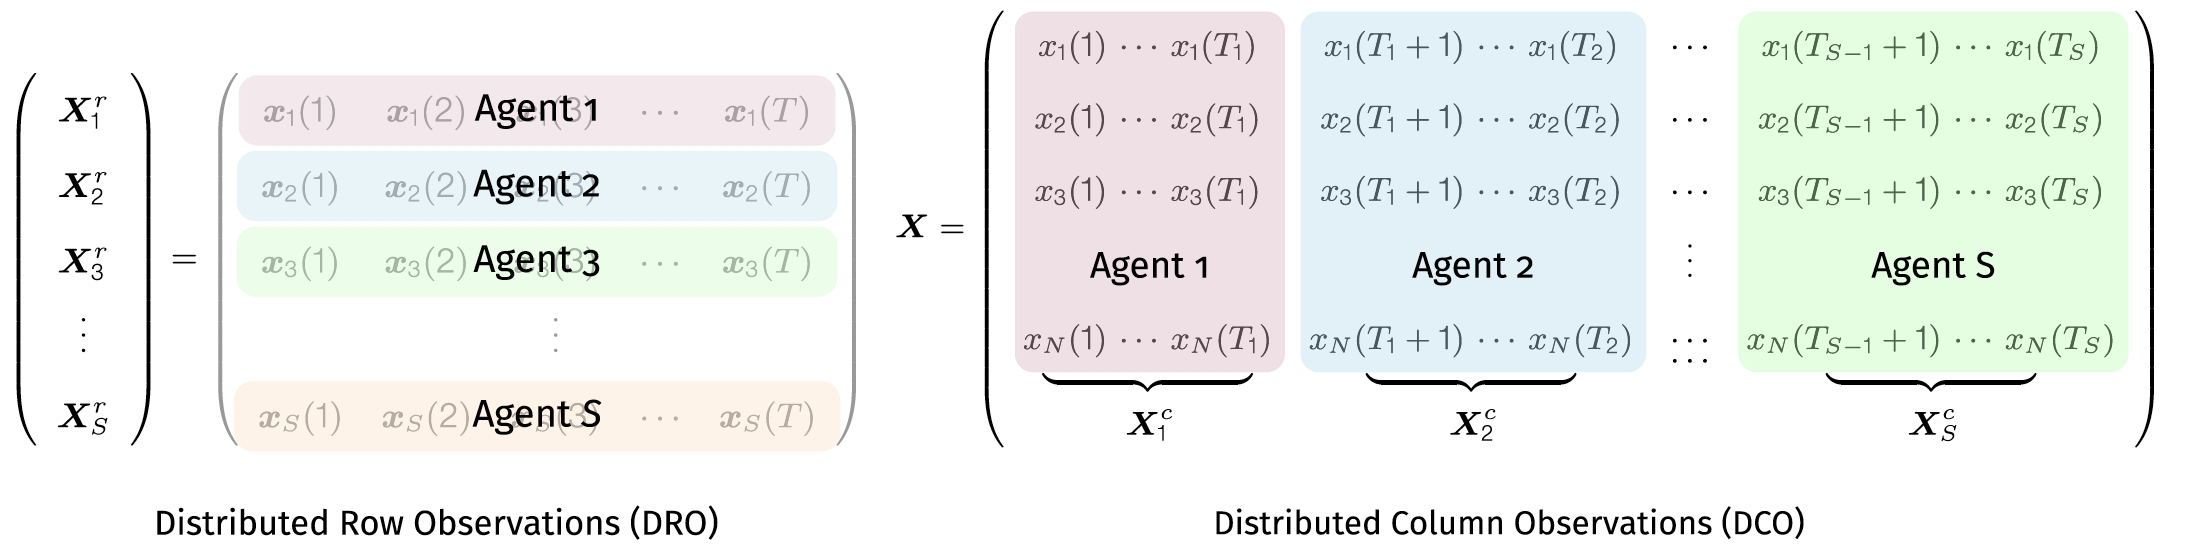
\includegraphics[width=12cm, height=4cm]{2.png}
		\caption{Data Model} 
		\label{Data Model}	
	\end{figure}	 
\end{frame}

\begin{frame}{Backgrounding}{Two Types of Data Model}
	 \begin{itemize}
	 	\item{
	 		The DCO setting assumes that each agent observes a subset of columns of $ X \in {C^{N*T}} $:
	 		\[X = (X_1^c,X_2^c,...,X_S^c)\]
	 		where $ X_i^c \in {C^{N*Ti}} $ is the column-partitioned sub-matrix and $ \sum\limits_{i = 1}^S {{T_i}}  = T $.
	 	}
		\item{
			DCO applies when high-dimension data are stored in different sites in a network.
		}
	 \end{itemize} 
\end{frame}

\begin{frame}{Backgrounding}{Two Types of Data Model}
	 \begin{itemize}
	 	\item{
	 	The DRO setting assumes that each agent observes only a subset of rows of $ X \in {C^{N*T}} $:
	 	\[X = {({(X_1^r)^T},{(X_2^r)^T},...,{(X_S^r)^T})^T}\]
	 	where $ X_i^r \in {C^{Ni*T}} $ is the column-partitioned sub-matrix and $ \sum\limits_{i = 1}^S {{N_i}}  = N $. 
	 	}
		\item{
			DRO applies when data have a multidimensional time series and each sample is distributed across the nodes.
		}
	 \end{itemize} 
\end{frame}


\begin{frame}{Backgrounding}{Two Types of Communication Model}
	 \begin{itemize}
		\item{
			The designs of D-PCA algorithms also differ in the types of communication among each node:
			\begin{enumerate}
  				\item master-slave type
  				\item mesh type
			\end{enumerate}
			\begin{figure}[ht]
				\centering
				%插入图形
				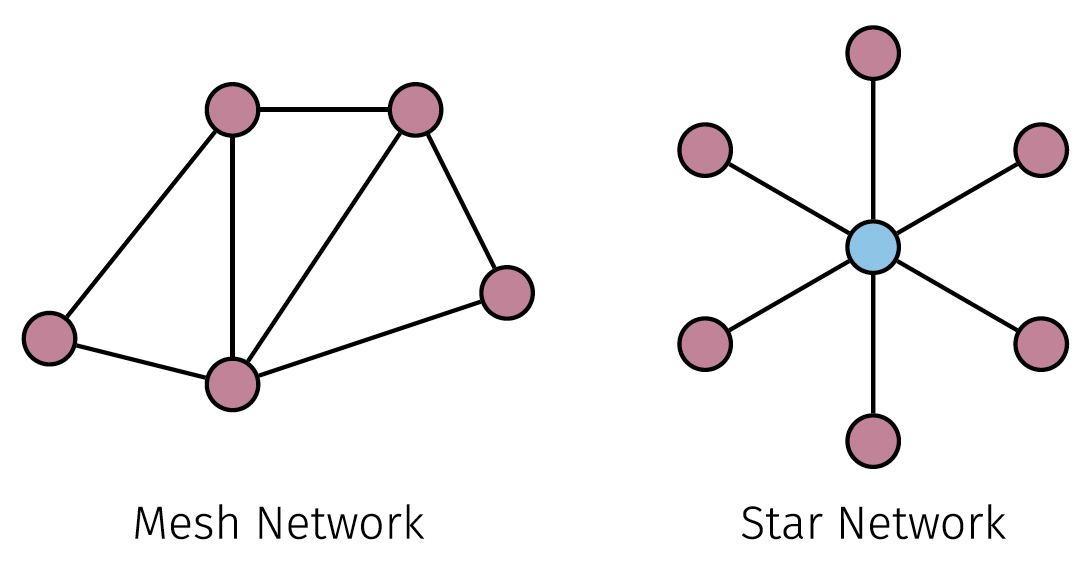
\includegraphics[width=10cm,height=4.5cm]{1.png}
				\caption{Communication Model} 
				\label{Communication Model}	
			\end{figure}
		}
	 \end{itemize}
\end{frame}


\begin{frame}{Backgrounding}{Two Types of Communication Model}
	 \begin{itemize}
		\item{
			How master-slave model work?
			\begin{enumerate}
			  \item in local stage, each slave node solves a local PCA
			  \item send local PCA results to the master node
			  \item in global stage, the master node computes the global PCA from the aggragated data
			\end{enumerate}
			%Master-slave model applies to DCO data.
		}
		\item{
			How mesh model work?
			\begin{enumerate}
			  \item all nodes and links perform the same function
			  \item all nodes exchange partial computations
			  \item transmitting information from one node to another may require multihop communications
			\end{enumerate}
			%Mesh model applies to DRO data.
		}
	 \end{itemize}
\end{frame}


\subsection{Average Consensus Algorithm}

\begin{frame}{Average Consensus Algorithm}
	\begin{itemize}
		\item{
			Why need Average Consensus(AC) Algorithm?
			
			In D-PCA algorithm, the key is to aggregate and share information across nodes.
			
			\begin{itemize}
				\item{
					For master-slave model, we can centralize information in master node.
				}
				\item{
					For mesh model, this has to be done with a sequence of computation steps adaptable to the network structure.
				}
			\end{itemize}
		
			
			We cannot centralize information directly in mesh model, so we take the iterative method to aggregate data。
		}
	\end{itemize}
\end{frame}

\begin{frame}{Average Consensus Algorithm}
	\begin{itemize}
		\item{
			Assume that the system of N sensor nodes is connected through a communication network. It is  modeled by a graph whose topology is represented by the corresponding Laplacian matrix L.\cite{1}
		}
		\item{
			The elements of matrix L \cite{2}
			\[{l_{ij}} = \left\{ \begin{gathered}
  {d_j},{\text{ }}i = j \hfill \\
   - 1,{\text{ }}i{\text{ communicates with j}} \hfill \\
  0,{\text{ else}} \hfill \\ 
\end{gathered}  \right.\]
			where $ {d}_{j} $ is the number of its neighbor.
		}
		\item{
		Let $ W = I - \varepsilon L $. The following linear iterative algorithm :
		\[{x_j}(t + 1) = {W_{jj}}{x_j}(t) + \sum\limits_{k \in N} {{W_{jk}}{x_k}(t)} \]
		\[x(t + 1) = Wx(t)\]
		}
	\end{itemize}
\end{frame}

\begin{frame}{Average Consensus Algorithm}
	\begin{itemize}
		\item{
			$ W1 = 1 $, so the eigenvector is 1 and eigenvalue is 1. The second largest eigenvalue of W, $ {\lambda _2} < 1 $. 
		}
		\item{
			No matter what the initial node values are, we must have
			\[\mathop {\lim }\limits_{t \to \infty } x(t) = \mathop {\lim }\limits_{t \to \infty } {W^t}x(0) = \frac{1}{n}{11^T}x(0)\]
		}
		\item{
		 	All elements in x(t) are the same, and are the average of x(0) elements.
			
		}
		\item{
			Therefore, by AC algorithm, each node only need to communicates with its neighbor nodes. After iteration,we can compute the average of all nodes.
		}
	\end{itemize}
\end{frame}


%\begin{frame}{Average Consensus Algorithm}
%	\begin{itemize}
%		\item{
%			We can compute $ {x_{avg}} $ distributively as follows.
%			\begin{algorithm}[H]
%			\begin{algorithmic}[1]
%			\STATE  Initialize as $ {Z_i}[0] = {x_i} $ for all i
%			
%			\FOR{$l=1$ to $L$}
%			\FOR{$i=1$ to $S$}
%			\STATE ${Z_i}[l] = \sum\limits_{j = 1}^N {{W_{ij}}[l]{Z_j}[l - 1]} $		
%			\ENDFOR
%			\ENDFOR
%			\end{algorithmic}
%			\caption{AC Algorithm}
%			\label{alg:1}
%			\end{algorithm}
%		}
%		\item{
%		The variable after the Lth update, as output of the above subroutine:
%		\[\{ {Z_i}[l]\} _{i = 1}^N = AC(\{ {x_i}\} _{i = 1}^S;L)\]
%		$ {Z_i}[l] = A{C_i}(\{ {x_i}\} _{i = 1}^S;L) $ denotes the output of the AC subroutine stored at the ith node.
%		}
%		
%	\end{itemize}
%
%\end{frame}

\subsection{Distributed PCA}

\begin{frame}{Distributed PCA}{PDMM for DCO}
\begin{itemize}
\item{
A distributed PCA method can be obtained by simply approximating the global correlation
matrix via the AC subroutine,
\begin{equation}
{{\hat{R}}_{u,i}}=N\cdot AC(\{{{u}_{i}}u_{i}^{T}\}_{i=1}^{N};L)\approx {{R}_{u}}
\end{equation}
}
\item{
In other words, each agent obtains an approximate of the global correlation matrix and the desired PCA can be then computed from ${{\hat{R}}_{u,i}}$.

}
\end{itemize}
\end{frame}



\begin{frame}{Distributed PCA}{PDMM for DCO}
\begin{itemize}
\item{
Eigenvalue decomposition of ${{R}_{x}}$ and reduce its dimension to p-dim.
\begin{equation}
{{R}_{u}}=\sum\limits_{i=1}^{N}{{{\lambda }_{i}}{{u}_{i}}u_{i}^{T}}\xrightarrow{\text{reduce dim}}{{R}_{u}}\approx \sum\limits_{i=1}^{P}{{{\lambda }_{i}}{{u}_{i}}u_{i}^{T}}
\end{equation}
}
\item{
Supposed that we have N distributed nodes, so the optimization problem is 
\begin{equation}
\begin{align}
  & \min \sum\limits_{i\in V}{-x_{i}^{T}{{R}_{u}}{{x}_{i}}} \\ 
 & s.t.\text{ }x_{_{i}}^{T}{{x}_{i}}=1,\text{ }i\in V \\ 
 & \text{     }{{x}_{i}}={{x}_{j}},\text{ }\forall (i,j)\in E \\ 
\end{align}
\end{equation}
}
\end{itemize}
\end{frame}

\begin{frame}{Distributed PCA}{PDMM for DCO}
\begin{itemize}
\item{
The PDMM \cite{8} solves problem in this form:
\begin{equation}
  \begin{align}
  & \min \sum\limits_{i\in V}{{{f}_{i}}(x)} \\ 
 & s.t.\text{ }{{A}_{ij}}{{x}_{i}}+{{A}_{ij}}{{x}_{j}}={{c}_{ij}},\text{ }\forall (i,j)\in E \\ 
\end{align}
\end{equation}
where 
\begin{equation}
  {{f}_{i}}(x)=-u_{i}^{T}{{R}_{x}}{{u}_{i}}
\end{equation}

\begin{equation}
\left\{ \begin{align}
  & {{A}_{ij}}=I,\text{ }i<j \\ 
 & {{A}_{ji}}=-I,\text{ others} \\ 
\end{align} \right.
\end{equation}
}
\begin{equation}
{{c}_{ij}}=0
\end{equation}

\end{itemize}
\end{frame}

\begin{frame}{Distributed PCA}{PDMM for DCO}
\begin{itemize}
\item{
	We denote $\delta $ as the Lagrangian multiplier, and the Lagrangian of this primal problem can be constructed as
\begin{equation}
{{L}_{p}}(x,\delta )=\sum\limits_{(i,j)\in E}{\delta _{ij}^{T}({{c}_{ij}}-{{A}_{ij}}{{x}_{i}}-{{A}_{ji}}{{x}_{j}})}+\sum\limits_{i\in V}{\left[ {{f}_{i}}({{x}_{i}})+\theta _{i}^{T}(1-x_{i}^{T}{{x}_{i}}) \right]}	
\end{equation}
}

\item{
	The Augmented Primal-Dual Lagrangian function is
\begin{equation}
{{L}_{P}}=\sum\limits_{i\in V}{\left[ {{f}_{i}}({{x}_{i}})-\sum\limits_{j\in N(i)}{\lambda _{j|i}^{T}({{A}_{ij}}{{x}_{i}}-{{c}_{ij}})}-f_{i}^{*}(A_{i}^{T}{{\lambda }_{i}}) \right]}+h({{x}_{i}},{{\lambda }_{i}})  
\end{equation}
where
\begin{equation}
h({{x}_{i}},{{\lambda }_{i}})=\sum\limits_{(i,j)\in E}{(\frac{1}{2}{{\left\| {{A}_{ij}}{{x}_{i}}+{{A}_{ji}}{{x}_{j}}+{{c}_{ij}} \right\|}^{2}}-\frac{1}{2}{{\left\| {{\lambda }_{i|j}}-{{\lambda }_{j|i}} \right\|}^{2}})}
\end{equation}
}
\end{itemize}
\end{frame}

\begin{frame}{Distributed PCA}{PDMM for DCO}
\begin{itemize}
\item{
At iteration k, the update scheme of PDMM is
\begin{equation}
\begin{align}
  & x_{i}^{k+1}=x_{i}^{k}-\alpha {{\nabla }_{{{x}_{i}}}}{{L}_{P}} \\ 
 & \theta _{i}^{k+1}=\theta _{i}^{k}+\alpha {{\nabla }_{{{\theta }_{i}}}}{{L}_{P}} \\ 
 & \lambda _{i|j}^{k+1}=\lambda _{i|j}^{k}+({{c}_{ij}}-{{A}_{ji}}x_{j}^{k}-{{A}_{ij}}x_{i}^{k}),\text{ }\forall i\in V,\text{ }j\in N(i) \\ 
\end{align}
\end{equation}
where
\begin{equation}
{{\nabla }_{{{x}_{i}}}}{{L}_{P}}=-2{{R}_{{{u}_{i}}}}{{x}_{i}}-\sum\limits_{j\in N(i)}{\lambda _{_{j|i}}^{T}{{A}_{ij}}}-2{{\theta }_{i}}{{x}_{i}}+\sum\limits_{(i,j)\in E}{{{A}_{ij}}({{A}_{ij}}{{x}_{i}}+{{A}_{ji}}{{x}_{j}})}
\end{equation}
\begin{equation}
 {{\nabla }_{{{\theta }_{i}}}}({{L}_{P}})=1-2x_{i}^{T}{{x}_{i}}
\end{equation}
}
\end{itemize}
\end{frame}

			
\begin{frame}{Distributed PCA}{PDMM for DCO}
			\begin{algorithm}[H]
			\begin{algorithmic}[1]
			\STATE  Initialize as $ x_{i}^{0} $, $\lambda _{i|j}^{0}$, $ \theta _{i}^{0}$ for all nodes		
			\FOR{$k=1$ to $K$}
			\FOR{$i=1$ to $N$}
			\STATE 	$\begin{gathered}
  x_i^{k + 1} = x_i^k - \alpha {\nabla _{{x_i}}}{L_P} \hfill \\
  \theta _i^{k + 1} = \theta _i^k + \alpha {\nabla _{{\theta _i}}}{L_P} \hfill \\
  \lambda _{i|j}^{k + 1} = \lambda _{i|j}^k + ({c_{ij}} - {A_{ji}}x_j^k - {A_{ij}}x_i^k),{\text{ }}\forall i \in V,{\text{ }}j \in N(i) \hfill \\ 
\end{gathered} $		\ENDFOR
			\ENDFOR
			\end{algorithmic}
			\caption{PDMM}
			\label{alg:1}
			\end{algorithm}

\end{frame}



			
\begin{frame}{Distributed PCA}{PDMM for DCO (Rayleigh Quotient)}
\begin{itemize}
\item{
We introduce Rayleigh quotient to replace the constrain $x_{_{i}}^{T}{{x}_{i}}=1$, and the optimization problem is 
\begin{equation}
\begin{align}
  & \min \sum\limits_{i\in V}{\frac{-x_{i}^{T}{{R}_{u}}{{x}_{i}}}{x_{i}^{T}{{x}_{i}}}} \\ 
 & s.t.\text{     }{{x}_{i}}={{x}_{j}},\text{ }\forall (i,j)\in E \\ 
\end{align}
\end{equation}
}
\end{itemize}
\end{frame}

\begin{frame}{Distributed PCA}{PDMM for DCO (Rayleigh Quotient)}
\begin{algorithm}[H]
			\begin{algorithmic}[1]
			\STATE  Initialize as $ x_{i}^{0} $, $\lambda _{i|j}^{0}$for all nodes		
			\FOR{$k=1$ to $K$}
			\FOR{$i=1$ to $N$}
			\STATE 	$\begin{gathered}
  x_i^{k + 1} = x_i^k - \alpha {\nabla _{{x_i}}}{L_P} \hfill \\
  \lambda _{i|j}^{k + 1} = \lambda _{i|j}^k + ({c_{ij}} - {A_{ji}}x_j^k - {A_{ij}}x_i^k),{\text{ }}\forall i \in V,{\text{ }}j \in N(i) \hfill \\ 
\end{gathered} $		\ENDFOR
			\ENDFOR
			\end{algorithmic}
			\caption{PDMM (Rayleigh Quotient)}
			\label{alg:1}
			\end{algorithm}

\end{frame}


\begin{frame}{Distributed PCA}{PDMM for DCO (Time-varing constrains)}
\begin{itemize}
\item{

\begin{equation}
\begin{align}
  & \min \sum\limits_{i\in V}{-x_{i}^{T}{{R}_{{{u}_{i}}}}}{{x}_{i}} \\ 
 & s.t.\text{ }{{A}_{ij}}{{x}_{i}}+{{A}_{ij}}{{x}_{j}}={{c}_{ij}},\text{ }\forall (i,j)\in E \\ 
\end{align}
\end{equation}
}
where at iteration k
\begin{equation}
 \left\{ \begin{align}
  & {{A}_{ij}}=I,\text{ }i<j \\ 
 & {{A}_{ij}}=-I,\text{ }i>j \\ 
 & {{A}_{ij}}=\left( \begin{matrix}
   x_{1}^{k-1} & \cdots  & x_{N}^{k-1}  \\
\end{matrix} \right),\text{ }i=j \\ 
\end{align} \right.
\end{equation}
\end{itemize}
\end{frame}



\begin{frame}{Distributed PCA}{PDMM for DCO (Time-varing constrains)}

\begin{algorithm}[H]
			\begin{algorithmic}[1]
			\STATE  Initialize as $ x_{i}^{0} $, $\lambda _{i|j}^{0}$, $ {A_{ii}}$ for all nodes		
			\FOR{$k=1$ to $K$}
			\FOR{$i=1$ to $N$}
			\STATE 	\[\begin{gathered}
  x_i^{k + 1} = x_i^k - \alpha {\nabla _{{x_i}}}{L_P} \hfill \\
  \lambda _{i|j}^{k + 1} = \lambda _{i|j}^k + ({c_{ij}} - {A_{ji}}x_j^k - {A_{ij}}x_i^k),{\text{ }}\forall i \in V,{\text{ }}j \in N(i) \hfill \\ 
\end{gathered} \]		\ENDFOR
	
\[{A_{ii}} = (\begin{array}{*{20}{c}}
  {x_1^{k - 1}}& \cdots &{x_N^{k - 1}} 
\end{array})\]

			\ENDFOR
			\end{algorithmic}
			\caption{PDMM (Time-varing constrains)}
			\label{alg:1}
			\end{algorithm}

\end{frame}



%\begin{frame}{Distributed PCA}{Distributed Power Method (DistPM) for DCO}
%	\begin{itemize}
%		\item{
%			Approximate of the global correlation matrix:
%			\[{\hat R_{x.i}} = \frac{S}{N} \cdot A{C_i}(\{ X_j^C{(X_j^C)^T}\} _{j = 1}^S;L) \approx {\hat R_x}\]
%		}
%		\item{
%			Use the Power method to compute EVD of $ {\hat R_x} $:
%			\[\begin{gathered}
%  {u_1}[k] = \frac{1}{N}X{X^T}{u_1}[k - 1] \\ 
%   = \frac{1}{T}\sum\limits_{i = 1}^S {(X_i^C{{(X_i^C)}^T}{u_1}[k - 1])}  \\ 
%\end{gathered} \]
%		}
%	\end{itemize}
%\end{frame}
%
%\begin{frame}{Distributed PCA}{Distributed Power Method (DistPM) for DCO}
%	\begin{itemize}
%		\item{
%			We can compute $ {x_{avg}} $ distributively as follows.
%			\begin{algorithm}[H]
%			\begin{algorithmic}[1]
%			\STATE  Initialize for each agent an independent random vector $ u_1^i[0] \in {C^N} $
%			
%			\FOR{$k=1$ to $K$}
%			\STATE For all nodes, perform the recursion
%			\[\begin{gathered}
%  u_1^i[k] = S \cdot A{C_i}(\{ X_j^C{(X_j^C)^T}\bar u_1^j[k - 1]\} _{j = 1}^S;L) \hfill \\
%  \bar u_1^i[k] = u_1^i[k]/\left\| {u_1^i[k]} \right\| \hfill \\ 
%\end{gathered} \]
%			\ENDFOR
%			\STATE Denote $ \hat u_i^i = \bar u_1^i[K] $ is the solution.
%			\end{algorithmic}
%			\caption{DistPM for DCO}
%			\label{alg:2}
%			\end{algorithm}
%		}
%		\item{
%			The sequence eigenvectors $ {{\hat u}_2},...,{{\hat u}_p} $ can be computed by the similar Power method.
%		}
%	\end{itemize}
%
%\end{frame}
%
%\begin{frame}{Distributed PCA}{Distributed Oja’s (D-Oja) Method for DRO}
%	\begin{itemize}
%		\item{
%			Define $ {u_{1,i}}[k] $ as approximate of the local eigenvector in ith node and approximate of the global eigenvector:
%			\[{u_1}[k] = \left( {\begin{array}{*{20}{c}}
%  {{u_{1,1}}[k]} \\ 
%   \vdots  \\ 
%  {{u_{1,S}}[k]} 
%\end{array}} \right)\]
%			
%			where \[{u_{1,i}}[k] \in {C^{{N_i}}},\sum\limits_{i = 1}^S {{N_i}}  = N\]
%		}
%		
%	\end{itemize}
%\end{frame}
%
%\begin{frame}{Distributed PCA}{Distributed Oja’s (D-Oja) Method for DRO}
%	\begin{itemize}
%		\item{
%			Use Oja method to solve EVD:
%			\[{u^{Oja}}(t + 1) = {u^{Oja}}(t) + {\gamma _t}[x(t){x^T}(t){u^{Oja}}(t) - {\left| {{x^T}(t){u^{Oja}}(t)} \right|^2} \cdot {u^{Oja}}(t)]\]
%		}
%		\item{
%			The inner product of $ {x^T}(t){u^{Oja}}(t) $ is computed from local terms available at each agent
%			\[{x^T}(t){u^{Oja}}(t) = \sum\limits_{i = 1}^S {x_i^T(t)u_i^{Oja}(t)}  \approx S \cdot A{C_i}(\{ x_j^T(t)u_j^{Oja}(t)\} _{j = 1}^S;L)\]
%		}
%	\end{itemize}
%\end{frame}
%
%\begin{frame}{Distributed PCA}{Distributed Oja’s (D-Oja) Method for DRO}
%	\begin{itemize}
%		\item{
%			The D-Oja’s method for DRO is summarized:
%			\begin{algorithm}[H]
%			\begin{algorithmic}[1]
%			\STATE  Initialize for each agent an independent random vector $ u_1^i[0] \in C^{{N_i}} $
%			\STATE For all nodes, perform the recursion
%			
%			\[pro{d_i}(t) = S \cdot A{C_i}(\{ x_j^T(t)u_j^{Oja}(t)\} _{j = 1}^S;L)\]
%			\[u_i^{Oja}(t + 1) = u_i^{Oja}(t) + {\gamma _t}(pro{d_i}(t) \cdot {x_i}(t) - {\left| {pro{d_i}(t)} \right|^2} \cdot u_i^{Oja}(t))\]
%			
%			\end{algorithmic}
%			\caption{D-Oja for DRO}
%			\label{alg:3}
%			\end{algorithm}
%		}
%	\end{itemize}
%
%\end{frame}

% You can reveal the parts of a slide one at a time
% with the \pause command:
%\begin{frame}{Second Slide Title}
%  \begin{itemize}
%  
%  \item {
%    First item.
%    \pause % The slide will pause after showing the first item
%  }
%  \item {   
%    Second item.
%  }
%  % You can also specify when the content should appear
%  % by using <n->:
%  \item<3-> {
%    Third item.
%  }
%  \item<4-> {
%    Fourth item.
%  }
%  % or you can use the \uncover command to reveal general
%  % content (not just \items):
%  \item<5-> {
%    Fifth item. \uncover<6->{Extra text in the fifth item.}
%  }
%  \end{itemize}
%\end{frame}

%\section{Second Main Section}
%
%\subsection{Another Subsection}
%
%\begin{frame}{Blocks}
%\begin{block}{Block Title}
%You can also highlight sections of your presentation in a block, with it's own title
%\end{block}
%\begin{theorem}
%There are separate environments for theorems, examples, definitions and proofs.
%\end{theorem}
%\begin{example}
%Here is an example of an example block.
%\end{example}
%\end{frame}
%
%% Placing a * after \section means it will not show in the
%% outline or table of contents.
%\section*{Summary}
%
%\begin{frame}{Summary}
%  \begin{itemize}
%  \item
%    The \alert{first main message} of your talk in one or two lines.
%  \item
%    The \alert{second main message} of your talk in one or two lines.
%  \item
%    Perhaps a \alert{third message}, but not more than that.
%  \end{itemize}
%  
%  \begin{itemize}
%  \item
%    Outlook
%    \begin{itemize}
%    \item
%      Something you haven't solved.
%    \item
%      Something else you haven't solved.
%    \end{itemize}
%  \end{itemize}
%\end{frame}



% All of the following is optional and typically not needed. 
\appendix
\section<presentation>*{\appendixname}
\subsection<presentation>*{For Further Reading}

\begin{frame}[allowframebreaks]
  \frametitle<presentation>{For Further Reading}
    
  \begin{thebibliography}{10}
    
  \beamertemplatebookbibitems
  % Start with overview books.
  \bibitem{6}
Benesty, Jacob, and Chen Jingdong. Study and design of differential microphone arrays. Vol. 6. Springer Science & Business Media, 2012.
\bibitem{7}
Benesty, Jacob, Jingdong Chen, and Israel Cohen. Design of Circular Differential Microphone Arrays. Vol. 12. Switzerland: Springer, 2015.
\bibitem{4}
Chatelin, Françoise, ed. Eigenvalues of Matrices: Revised Edition. Society for Industrial and Applied Mathematics, 2012.

\beamertemplatearticlebibitems
  % Followed by interesting articles. Keep the list short. 

	  \bibitem{1}
    Wu, Sissi Xiaoxiao, et al. "A Review of Distributed Algorithms for Principal Component Analysis." Proceedings of the IEEE 106.8 (2018): 1321-1340.

  \bibitem{2}
Scaglione, Anna, Roberto Pagliari, and Hamid Krim. "The decentralized estimation of the sample covariance." 2008 42nd Asilomar Conference on Signals, Systems and Computers. IEEE, 2008.

\bibitem{3}
Qu, Yongming, et al. "Principal component analysis for dimension reduction in massive distributed data sets." Proceedings of IEEE International Conference on Data Mining (ICDM). 2002.
\bibitem{8}
Zhang, Guoqiang, and Richard Heusdens. "Bi-alternating direction method of multipliers over graphs." 2015 IEEE International Conference on Acoustics, Speech and Signal Processing (ICASSP). IEEE, 2015.  
  
  \end{thebibliography}

\end{frame}






\end{document}


